\chapter{Results from Testing of Global Model}
\label{appendix:A}
\section{Static Configuration Without Current}

\begin{figure}[H]
\centering
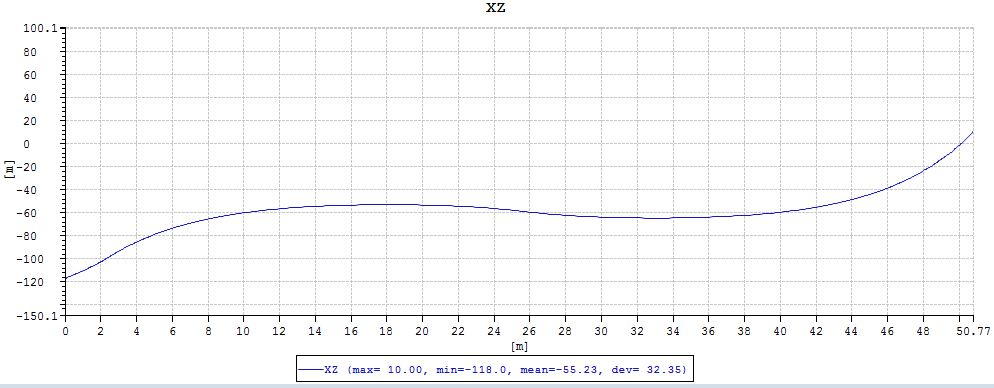
\includegraphics[scale=0.5]{figures/confignear}
\caption{Configuration for near position without current}
 \label{fig:confignear}
\end{figure}

\begin{figure}[H]
\centering
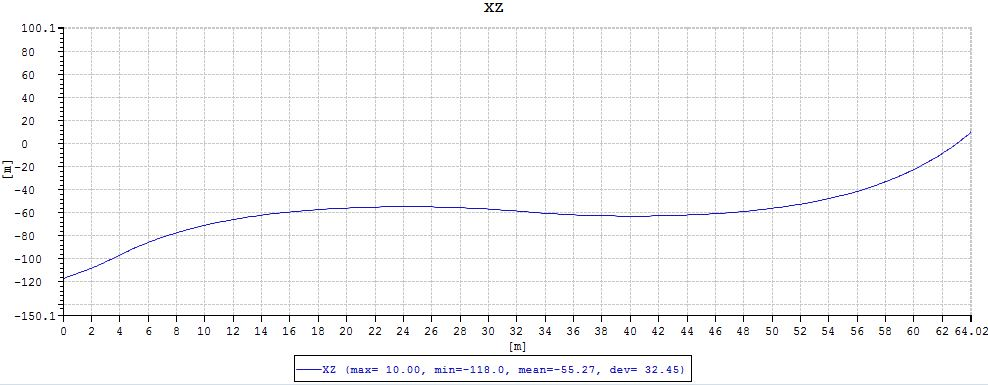
\includegraphics[scale=0.5]{figures/configneu}
\caption{Configuration for neutral position without current}
 \label{fig:configneu}
\end{figure}

\begin{figure}[H]
\centering
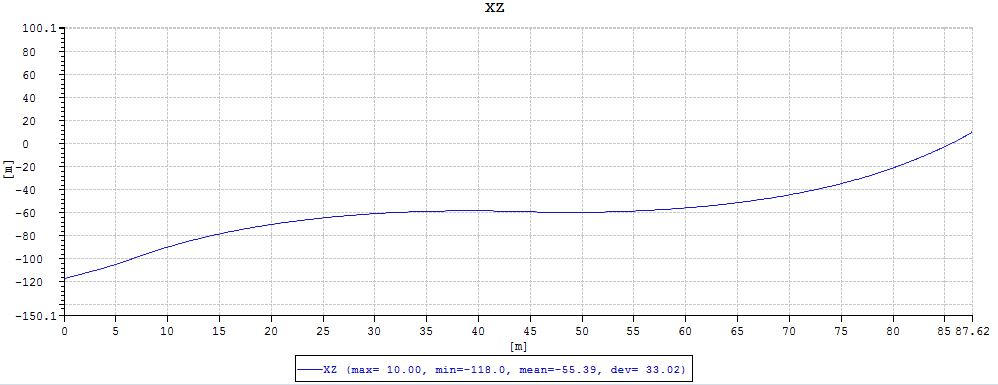
\includegraphics[scale=0.5]{figures/configfar}
\caption{Configuration for far position without current}
 \label{fig:configfar}
\end{figure}

\section{Static Configuration With Current}
\begin{figure}[H]
\centering
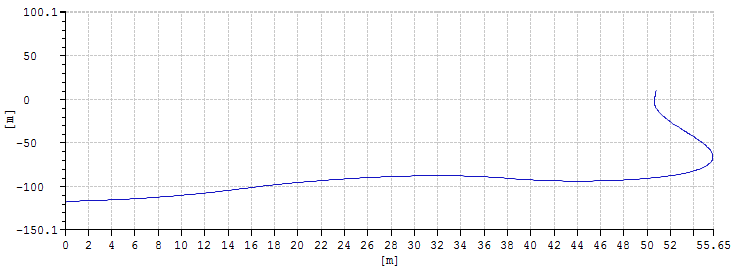
\includegraphics[scale=0.5]{figures/confignearc}
\caption{Configuration for near position with current}
 \label{fig:confignear}
\end{figure}

\begin{figure}[H]
\centering
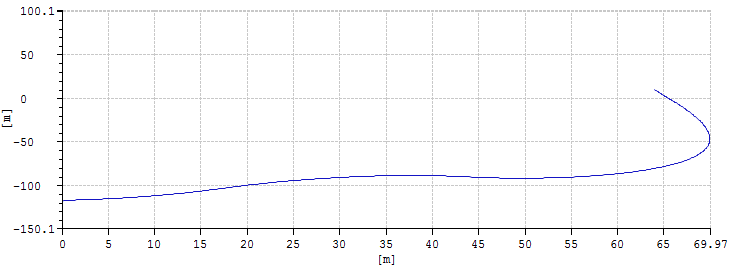
\includegraphics[scale=0.5]{figures/configneuc}
\caption{Configuration for neutral position with current}
 \label{fig:configneu}
\end{figure}

\begin{figure}[H]
\centering
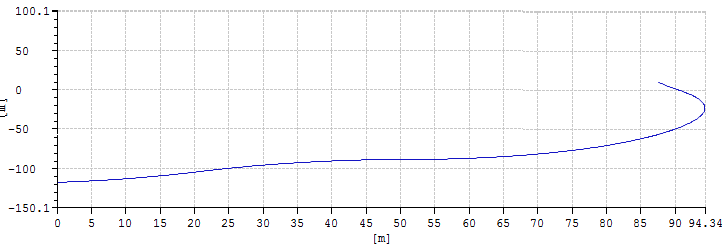
\includegraphics[scale=0.5]{figures/configfarc}
\caption{Configuration for far position with current}
 \label{fig:configfar}
\end{figure}

\section{Curvature}

\begin{figure}[H]
\centering
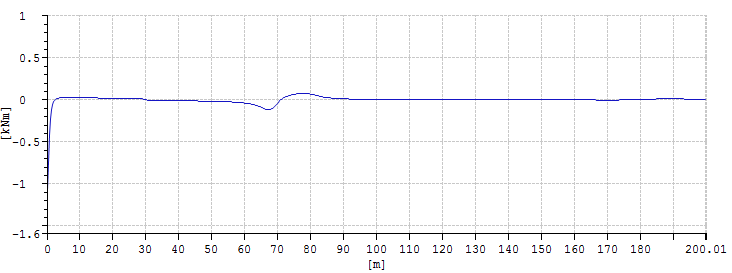
\includegraphics[scale=0.5]{figures/envcurvenear}
\caption{Curvature envelope for near position}
 \label{fig:envcurvenear}
\end{figure}

\begin{figure}[H]
\centering
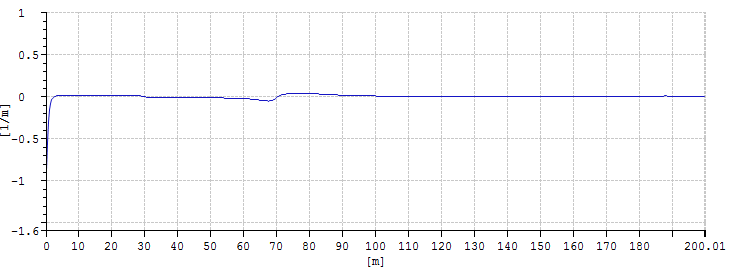
\includegraphics[scale=0.5]{figures/envcurveneu}
\caption{Curvature envelope for neutral position}
 \label{fig:envcurveneu}
\end{figure}

\begin{figure}[H]
\centering
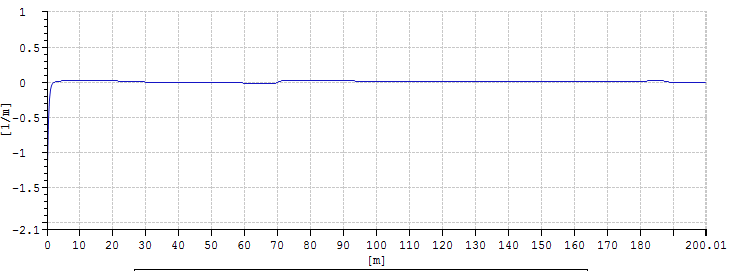
\includegraphics[scale=0.5]{figures/envcurvefar}
\caption{Curvature envelope for far position}
 \label{fig:envcurvefar}
\end{figure}

\section{Max Tension}

\begin{figure}[H]
\centering
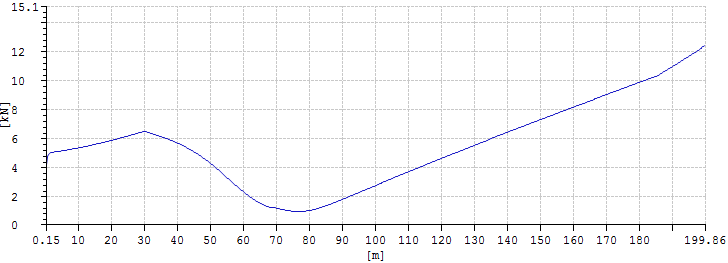
\includegraphics[scale=0.5]{figures/fmaxnear}
\caption{The max tension over the length of the cable in near position}
 \label{fig:fmaxnear}
\end{figure}


\begin{figure}[H]
\centering
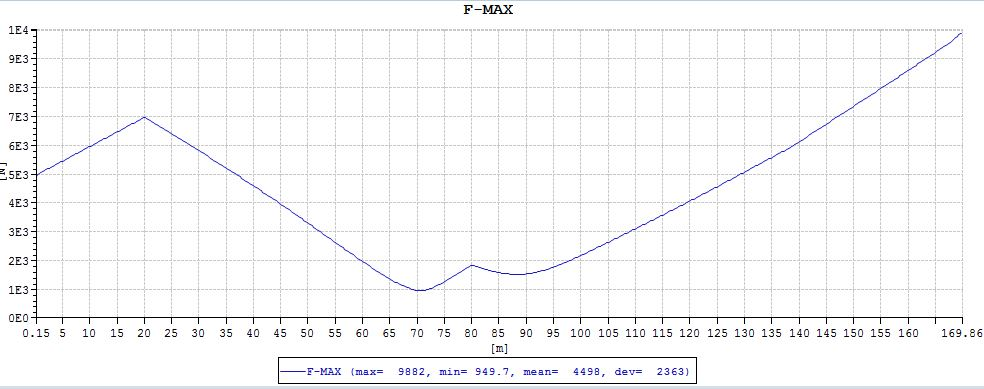
\includegraphics[scale=0.5]{figures/fmaxneu}
\caption{The max tension over the length of the cable in neutral position}
 \label{fig:fmaxneu}
\end{figure}


\begin{figure}[H]
\centering
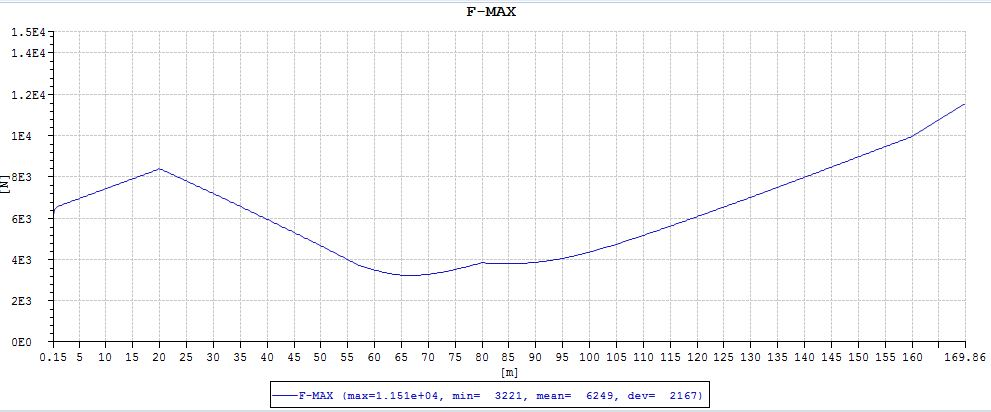
\includegraphics[scale=0.5]{figures/fmaxfar}
\caption{The max tension over the length of the cable in far position}
 \label{fig:fmaxfar}
\end{figure}

\section{Min Tension}

\begin{figure}[H]
\centering
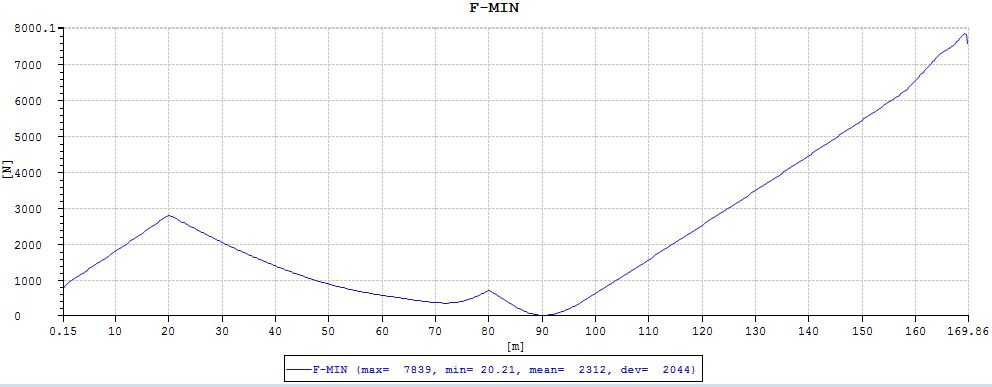
\includegraphics[scale=0.5]{figures/fminnear}
\caption{The minimum tension over the length of the cable in near position}
 \label{fig:fminnear}
\end{figure}


\begin{figure}[H]
\centering
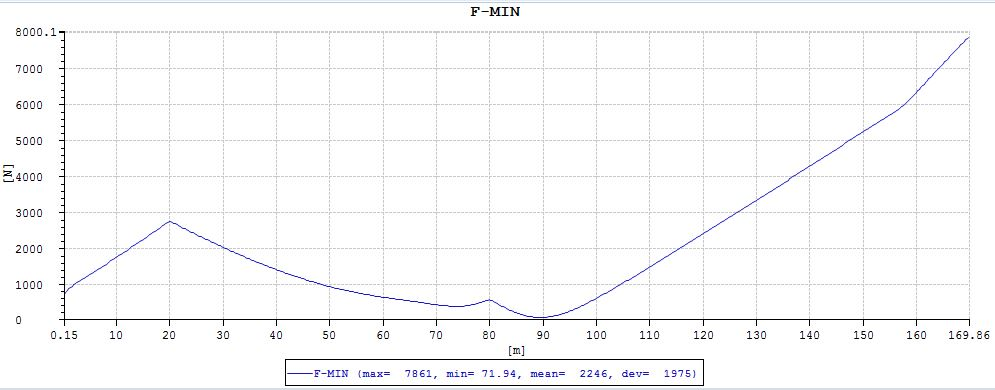
\includegraphics[scale=0.5]{figures/fminneu}
\caption{The minimum tension over the length of the cable in neutral position}
 \label{fig:fminneu}
\end{figure}


\begin{figure}[H]
\centering
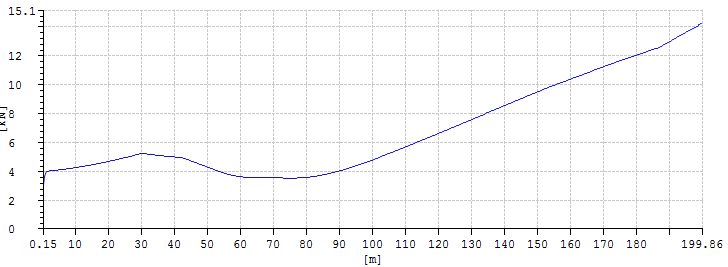
\includegraphics[scale=0.5]{figures/fminfar}
\caption{The minimum tension over the length of the cable in far position}
 \label{fig:fminfar}
\end{figure}



